\section{Синтаксический анализ контекстно-свободной аппроксимации}

Наш алгоритм принимает на вход управляющие таблицы LL-анализа, построенные по эталонной грамматике, и GFG, который является представлением КС-грамматики --- аппроксимации множества значений выражения. 
Мы переиспользуем основные структуры данных и функции описанного ранее алгоритма анализа регулярной аппроксимации на основе GLL, расширяя данный подход для корректной обработки GFG.

Алгоритм последовательно обходит узлы GFG, производя синтаксический анализ порождаемых им строк. 
Для правильного построения таких строк, согласно определению выводимости строки в GFG-грамматике, для каждого просматриваемого пути необходимо поддерживать баланс call- и return-узлов. 
То есть, при прохождении пути алгоритм должен манипулировать дополнительным стеком (назовем его \textit{CR-стеком}). 
При достижении call-узла в стек добавляется номер return-узла, соответствующего ему; при достижении end-узла необходимо снять со стека номер return-узла и продолжить обход из него. 

Для экономии памяти мы не храним CR-стек для каждой из текущих ветвей работы алгоритма (напомним, что GLL-алгоритм может одновременно рассматривать несколько вариантов разбора строки). 
Вместо этого множество CR-стеков, по аналогии с основным стеком GLL-анализатора, представляется в виде GSS. 
Пример можно увидеть на рисунке \ref{fig:gss}. GSS позволяет хранить только одну копию общих префиксов нескольких стеков, каждый путь в нем соответствует отдельному CR-стеку.

\begin{figure}[h]
	\centering
	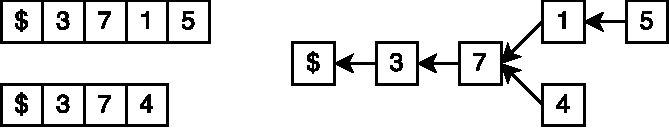
\includegraphics[width=6cm]{pictures/gss_cr}
	\caption{Структурированный в виде графа стек}
	\label{fig:gss}
\end{figure}

Для хранения указателя на текущую вершину стека мы добавили в дескрипторы дополнительное поле. 
Таким образом, дескриптором в нашем алгоритме называется пятерка вида $(L, u, i, N, s)$, где $i$ --- номер вершины GFG, $s$ --- указатель на вершину CR-стека в GSS, остальные поля аналогичны тем, которые представлены в дескрипторах оригинального GLL-алгоритма.

Другой особенностью работы с GFG является то, что он, в отличие от регулярной аппроксимации --- детерминированного конечного автомата, допускает возможность неоднозначного выбора пути обхода. 
Подобная ситуация возникает при наличии в исходной грамматике нескольких продукций, содержащих в левой части одинаковый нетерминал. 
Например, GFG на рисунке \ref{fig:gfg} содержит start-узел под номером 3, из которого выходит два ребра с пустой меткой (аналог $\epsilon$-переходов в конечном автомате).

Механизм дескрипторов позволяет решать проблему недетерминированного выбора пути --- для каждого из возможных вариантов создается отдельный дескриптор, который добавляется в очередь исполнения. 
Вернемся к примеру с узлом 3 на рисунке \ref{fig:gfg}. Пусть в текущий момент времени мы имеем дескриптор $(L_1, u_1, i_1, N_1, s_1)$. 
При рассмотрении ребер, выходящих из узла 3, будут созданы дескрипторы $(L_1, u_1, 4, N_1, s_1)$ и $(L_1, u_1, 5, N_1, s_1)$. Если ранее такие дескрипторы не создавались (для контроля за этим в GLL поддерживается глобальное множество создаваемых дескрипторов), они будут добавлены в очередь.

Функции \textbf{dispatcher} и \textbf{add} (проверка и добавление в очередь дескриптора) алгоритма анализа регулярной аппроксимации были незначительно изменены нами для работы с расширенными дескрипторами. 
Функция \textbf{processing} и методы для работы с основным стеком и построения SPPF переиспользованы без изменений.
Обработка start/call/exit-узлов и контроль за состоянием CR-стеков были реализованы во вспомогательной функции \textbf{closure}, псевдокод которой приведен ниже.
Она исполняется перед вызовами \textbf{dispatcher} и \textbf{processing}, производя рекурсивный обход GFG до тех пор, пока не встретит start- или scan-узел. 
При достижении start-узла создаются дескрипторы для каждого из возможных путей, и управление переходит к \textbf{dispatcher};
scan-узел обрабатывается функцией \textbf{processing} так же, как и вершина конечного автомата в оригинальном алгоритме.

\section{Closure properties of languages with polynomial rational indices}
\label{sec:closure}
Given a context-free language $L$ with a polynomial rational index, it is interesting to find which language operations preserve this property.  Boasson et al. \cite{RatBasic} give following useful relations for polynomial indices of two languages $L$ and $L'$.
\begin{theorem}[\cite{RatBasic}]
Context-free languages with polynomial rational indices are closed under intersection with a regular language, union, concatenation, homomorphism and inverse homomorphism. More precisely,
\begin{itemize}
\item $\rho_{L \cup L'} \le  \max{(\rho_L, \rho_{L'})} $
\item $\rho_{LL'} \le \rho_L + \rho_{L'}$
\item $\rho_{L \cap R}(n) \le \rho_L(nm)$, where $R$ is a regular language recognised by an $m$-state automaton
\item $\rho_{h(L)}(n) \le \rho_L(n)$ and $\rho_{h^{-1}(L)}(n) < n(\rho_L(n) +1)$, where $h: \Sigma^* \rightarrow \Delta^*$ is a homomorphism.
\end{itemize}
\end{theorem}
From the relations above it is easy to see that the family of context-free languages with polynomial rational indices is a full trio. Every full trio is closed under prefix and quotient with regular languages. Obviously, CFLs with polynomial rational indices languages are closed under reversal.  Next we show that context-free languages with polynomial rational indices are closed under Kleene star and insertion of a regular language (or context-free language with a polynomial rational index).
\begin{theorem}
Context-free languages with polynomial rational indices are closed under Kleene star and insertion of a regular language  (or context-free language with a polynomial rational index). Particularly,
\begin{itemize}
\item $\rho_{L^*}(n) \le n(\rho_L(n))$
\item $\rho_{LL'} \le \rho_L + \rho_{L'}$
\end{itemize}
\end{theorem}
\begin{proof}
\textit{Kleene star.} Let $G = (\Sigma, N, P, S)$ and $L(G)$ be a language with polynomial rational index. Consider language $L^{+}$, which grammar $G_1$ has the start nonterminal $S_1$. By definition of the Kleene plus operation, a rightmost derivation from $S_1$ generates a sequence of one or more start nonterminals $S$ from $G$, each of which generates some string in $L(G)$. Let $D$ be a directed labelled graph with $n$ nodes. Suppose there are nodes $u$ and $v$ in $D$ such that:
\begin{enumerate}
\item $v$ is not $L(G)$-reachable from $u$ and
\item $v$ is  $L^+$-reachable from $u$
\end{enumerate}
Then $v$ is reachable from $u$ via concatenation of words in $L(G)$. Consider the longest shortest path $u\pi_1 v$ between $u$ and $v$. It can be obtained by joining $(S, u, i), (S, i, j), ..., (S, w, v)$ into $(S_1, u, v)$.  If $L$ has the polynomial rational index, then for every realizable triple $(A, i, j)$ corresponding shortest path $i \pi j$ has at most polynomial length. There are no more than $O(n)$ such triples in concatenation because there are no repetitions of the same node in the sequence of start and end nodes of triples (otherwise $u\pi_1 v$ is not the shortest path, for example, path $u \rightarrow i \rightarrow k \rightarrow l \rightarrow i \rightarrow j \rightarrow v$ can be replaced with shorter path $u \rightarrow i  \rightarrow j \rightarrow v$), so $u\pi_1 v$ has at most polynomial length. In other words, we have $\rho_{L^+}(n) \le n(\rho_L(n))$.
\\
Family of languages with polynomial rational indices is a full trio closed under union, concatenation and Kleene star, therefore it is a full ALF. Full AFLs is known to be closed under substitution.
\\
\textit{Insertion of a regular language.} To prove closure under insertion of a regular language, the following PDA can be constructed. Let $L$ be a context-free language with polynomial rational index and let $M$ be a PDA recognizing $L$. New PDA $M'$ for insertion of a regular language $R$ recognized by finite automation $F$ into $L$ can be obtained as follows: duplicate all states in $M$, initial state is placed in first set and final states reside in the second set. Every state in the first set has its own copy of outgoing arcs of the initial state of $F$. Every ingoing arc of final state of $F$ is connected directly to every state of the second set of $M$. In other words, every state from the first set is the initial state of $F$ and every state from the second set is a final state of $F$. All arcs from $F$ are labelled the same way as they are labelled in $F$.
Consider intersection of $M'$ and arbitrary finite automotion $F'$ with $n$ states. The longest non-empty shortest path $i \pi j$ in the intersection of $M'$ and $F'$ consists of three sub-paths: $i\pi_1k$, $k\pi_2m$ and $m\pi_3j$, where $i\pi_1k$ ($m\pi_3j$) is the shortest paths in the intersection of $F'$ and first (second) set of states of $M$ respectively, and $k\pi_2m$ is the shortest path in the intersection of $F'$ and $F$. $k\pi_2m$ has at most polynomial length because all regular languges have polynomial rational indices, $i\pi_1k$ and $m\pi_3j$ have polynomial length because $M$ is a PDA for language with rational index, therefore  $i \pi j$ has polynomial length.
\end{proof}


Using closure properties, it is easier to find new subclasses of context-free languages for which CFL-reachability problem is in NC.
\begin{example}[Metalinear languages \cite{metalinear}.]
\\
Let $G = (\Sigma, N, P, S)$ be a context-free grammar. $G$ is \textit{metalinear} if all productions of $P$ are of the following forms:
\begin{enumerate}
\item $S \rightarrow A_1A_2...A_k$, where $A_i \in N - \{S\}$
\item $A \rightarrow u$, where $A \in N \setminus \{S\}$ and $u \in (\Sigma^*((N \setminus \{S\}) \cup {\varepsilon})\Sigma^*)$
\end{enumerate}


The width of a metalinear grammar is $max\{k$ | $S \rightarrow A_1A_2...A_k \}$. Metalinear languages of width 1 are obviously linear languages. It is easy to see that every metalinear language is a union of concatenations of $k$ linear languages. Linear languages have polynomial rational index,  CFLs with polynomial rational index are closed under concatenation and union, so metalinear languages have polynomial rational index.
\end{example}



Результатом работы алгоритма является SPPF, представляющий набор деревьев разбора строк, порождаемых GFG и одновременно с этим выводимых в эталонной грамматике.
Отметим, что SPPF может быть построен не всегда, так как класс КС-языков не замкнут относительно пересечения.